\chapter{Wstęp}

\section{Cele projektu}
Celem projektu jest stworzenie systemu wspomagającego obsługę kina w oparciu o rozproszoną i obiektową bazę danych. System będzie umożliwiać zarządzanie kinem – z wykorzystaniem relacyjnych baz danych replikujących miedzy sobą dane. W pojedynczym węźle bazy danych zawarte będą tabele opisujące miedzy innymi – seanse filmowe, przydział ich do poszczególnych sal kinowych. Aplikacja będzie umożliwiać ponadto tworzenie nowych wpisów w zależności od rodzaju użytkownika obsługującego program. Pracownik kina będzie wprowadzać nowe seanse do bazy; podczas bezpośredniej sprzedażny biletów będzie również wykreślał miejsca
na sali już zajęte – miejsca zawarte na biletach, poszukiwanie rezerwacji wykonanej na konkretna osobę (po imieniu lub nazwisku, czy tez numerze rezerwacji). Użytkownik(Klient) będzie mógł rezerwować konkretne miejsce na określony seans.

\section{Założenia projektowe}
Projekt został wykonany przy użyciu MySQL 5.7. Rozproszoność systemu oparta została o kontenery programu docker, na których skonfigurowane zostały węzły zarówno \textit{slave} jak i \textit{master}. W trakcie realizacji projektu zostały wykorzystane mechanizmy replikacji master-slave oraz master-slave z opóźnieniem. Do wykonania projektu bazy danych wykorzystane zostało narzędzie Microsoft Visio. Zarządzanie bazą danych odbywało się z poziomu narzędzia zwanego phpMyAdmin. Aplikacja kliencka została wykonana w technologii webowej, z wykorzystaniem platformy programistycznej Angular2 oraz języka programowania TypeScript. Komunikacja między bazą danych a aplikacją kliencką zapewnia API REST-owe napisane w języku PHP. \\

System składa się z:
\begin{itemize}
	\item jednego węzła master;
	\item trzech zwyczajnych węzłów slave;
	\item jednego węzła slave z opóźnieniem;
	\item aplikacji klienckiej;
	\item API REST-owego.
\end{itemize}

API REST-owe dodaje dane wysłane z aplikacji klienckiej do węzła master, natomiast odczyt danych dokonuje się losowo z jednego z trzech zwyczajnych węzłów slave. Węzeł opóźniony służy jako kopia zapasowa danych, głównie na wypadek wystąpienia poleceń typu DROP w węźle master. Struktura systemu została przedstawiona na rysunku~\ref{fig:diagram}.

\begin{figure} [H]
	\centering
	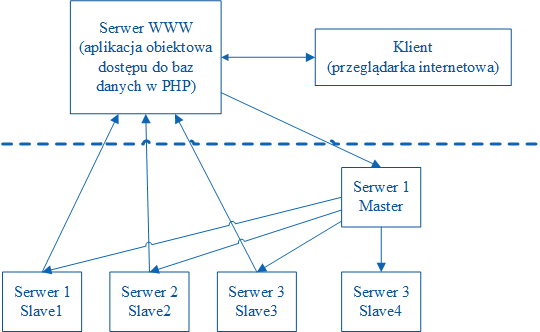
\includegraphics[width=0.6\linewidth]{rozdzial01/diagram.png}
	\caption{Struktura systemu}
	\label{fig:diagram}
\end{figure}

\section{Zakres projektu}
Zakres projektu dotyczy zaprojektowania i implementacji rozproszonego systemu bazodanowego dla kina. Projekt składa sę z kilku etapów.

\begin{itemize}
	\item Określenie wymagań funkcjonalnych aplikacji bazodanowej
	\item Testowanie mechanizmów replikacji oraz rozpraszania danych
	\item Opracowanie modelu konceptualnego i fizycznego bazy danych
	\item Implementacja bazy danych, procedur i widoków
	\item Projektowanie i implementacja aplikacji klienckiej
	\item Wdrożenie i testowanie aplikacji klienckiej
\end{itemize}

